%!TEX encoding = IsoLatin

%% Document is article 
\documentclass[a4paper]{article}

%% ----------------------------------------------------- PACKAGES ----------------------------------------------------- %%
\usepackage{coolArticle}
\usepackage[ruled]{algorithm2e}


%% ---------------------------------------------------- DOCUMENT ---------------------------------------------------- %%
\begin{document}

\noindent \textsc{Gallois-Montbrun} Gr�goire\\
\textsc{Faury} Louis 
	\titlebox{0.6}{Model Predictive Control}{Exercise \#3 - \textcolor{blue}{Group 2}}
	
	\section{Ex.1 : Computing invariant sets}
	{
		\paragraph{} We consider the following discrete time linear time-invariant system : 
		\begin{equation}
			x^+ = Ax 
		\end{equation}
		with : 
		\begin{equation}
			A = \begin{bmatrix} \cos{(\alpha)} & \sin{(\alpha)} \\ -\sin{(\alpha)} & cos{(\alpha)} \end{bmatrix} \beta
		\end{equation}
		and $\beta = 0.6$ and $\alpha = \frac{\pi}{6}$. 
		We also introduce the constraint set :
		\begin{equation}
			\mathbb{X} = \left\{ x\, \vert \, Hx \leq h\right\} \quad \text{ where } H = \begin{bmatrix} \cos{(\pi/3)} & \sin{(\pi/3)} \\ -\cos{(\pi/3)} & -\sin{(\pi/3)} \\ \sin{(\pi/3)} & -\cos{(\pi/3)} \\ -\sin{(\pi/3)} & \cos{(\pi/3)} \end{bmatrix} \, \text{ and } h = \begin{bmatrix}  2 & 1 & 2 & 5 \end{bmatrix}^T
		\end{equation}

		\paragraph{} $\color{red}\blacktriangleright$ We are going to implement the following algorithm : 
		\vspace{10pt}	
			
		\begin{algorithm}[H]
			\SetKwRepeat{Do}{do}{while}
	 		\SetAlgoLined
			\KwData{$\mathbb{X}$, $A$} 
			\KwResult{$\mathcal{O}_{\infty}$} 
			1.  Initialize : $\Omega_0 = \mathbb{X}$ \\
			2. \Do{$\Omega_{i+1}=\Omega_i$}
			{
				$\Omega_{i+1} = pre(\Omega_i)\cap \Omega_i $
			}
			3. $\mathcal{O}_{\infty} = \Omega_i$
			\caption{Maximum invariant set computation}
		\end{algorithm}
		\vspace{10pt}
		
		\noindent in order to compute the maximum invariant set contained in $\mathbb{X}$. The computations are made tractable by the linearity of our transition model as well as by the polytopal description of our different sets. The Matlab code performing this operations is provided with this report. 
		
		\begin{figure}[h!]
			\begin{minipage}{0.5\linewidth}
			{
				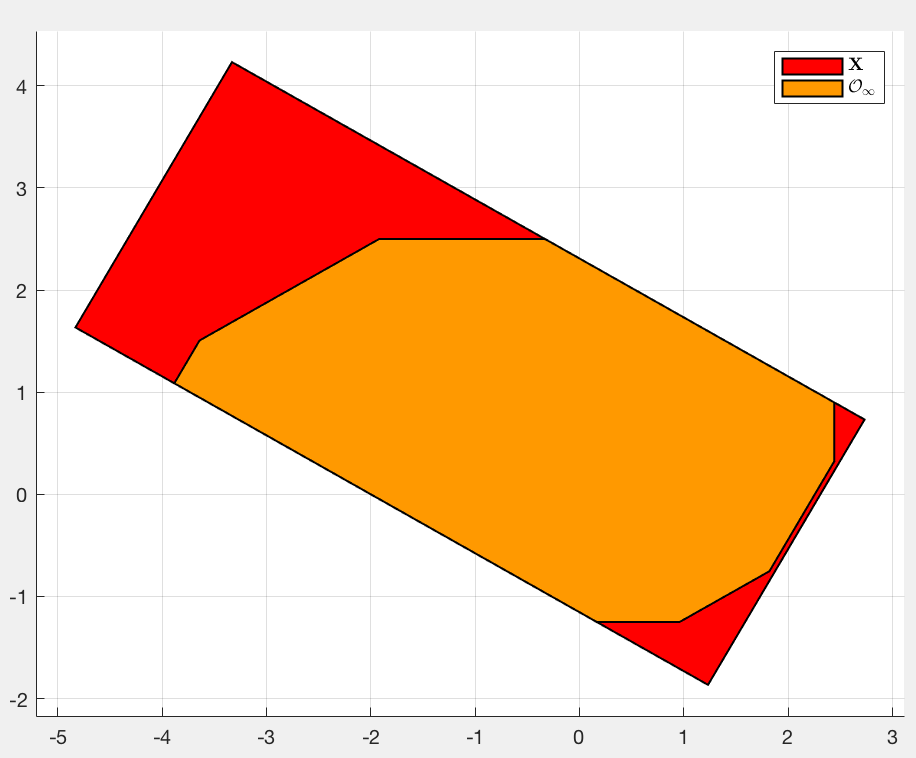
\includegraphics[width=0.95\linewidth]{feasible_set}
				\label{fig::max_inv}
				\caption{Feasible and maximum invariant set}
			}
			\end{minipage}
			\begin{minipage}{0.5\linewidth}
			{
				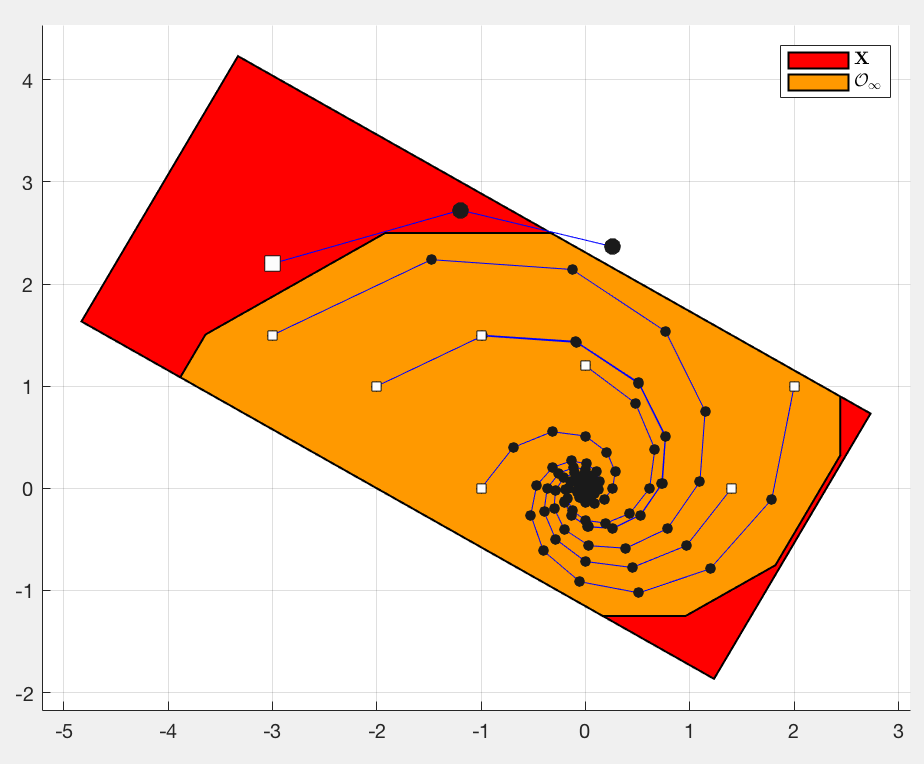
\includegraphics[width=0.95\linewidth]{feasible_traj}
				\label{fig::traj}
				\caption{Trajectories plot}
			}
			\end{minipage}
		\end{figure}
		
		\paragraph{} $\color{red}\blacktriangleright$ Figure (\ref{fig::max_inv}) displays the maximum invariant set as well as the feasible set. Figure (\ref{fig::traj}) plots 6 different trajectories starting in $\mathcal{O}_\infty$ as well as one trajectory starting in $\mathbb{X}\backslash\mathcal{O}_\infty$. One can notice that as expected, all trajectory starting in $\mathcal{O}_\infty$ remains in that set (and hence remain feasible) for all time, as they converge towards the origin. On the other hand, we notice that the only trajectory starting outside of the maximum invariant set quickly leaves the feasible set. 
	} 
		
	\section{Ex.2 : Computing controlled invariant sets}
	{
	
	}
	
	\section{Ex.3 : Q\&A}
	{
		\paragraph{} We hereinafter consider the system : 
		\begin{equation}
			x^+ = f(x,u) \quad (x,u)\in\mathbb{X}\times\mathbb{U}
		\end{equation}
		
		\begin{enumerate}
			\item If $A$ is the maximum invariant set for 
			\begin{equation}
				x^+ = f(x,\mu(x)) 
			\end{equation}
			therefore $A\subseteq B$ where $B$ is the maximum control invariant set for $f(x,u)$. Indeed, $A$ correspond to a particular case of $B$ where we consider a feedback controller, whereas in $B$ all kinds of control laws can be considerer. Therefore : 
			\begin{equation}
				\forall x \in A, \, \mathcal{X}(x,t) \in B \text{ for all } t>0
			\end{equation}
			where $\mathcal{X}(x,t)$ denotes the flow of the solution starting at $x$ for $t=0$. Therefore 
			\begin{equation}
				\color{red}
				A \subseteq B
			\end{equation}
		\end{enumerate}
	}
	
	
\end{document}